\section{Construction Algorithm}\label{algorithms}

%Android uses observer pattern to handle both user-driven and system-driven callbacks, namely non-lifecycle callbacks according to section \ref{background}. A non-lifecycle callback (termed as \begin{math} \mathcal{C} \end{math}) becomes valid only when its container listener is properly registered. Whereas the register process(termed as \begin{math} \mathcal{R} \end{math}) is located in another container callback (termed as \begin{math} \mathcal{P} \end{math}). 
%Define 0 callback status  (inactive, active, invoked)
%Define 1 register-triple
%The triple (\begin{math} \mathcal{P},\mathcal{R},\mathcal{C} \end{math})) named register-triple performs the key flow relations between callbacks, where the register process acts as a bridge connecting with two callbacks. Figure 2 illustrates the register-triple within the motivating example. ... Then we can define a generalized connection triple.
%Define 2 connection triple
%connection triple = register-triple + ICC connection

%\begin{figure}[!t]  
%  \centering  
%  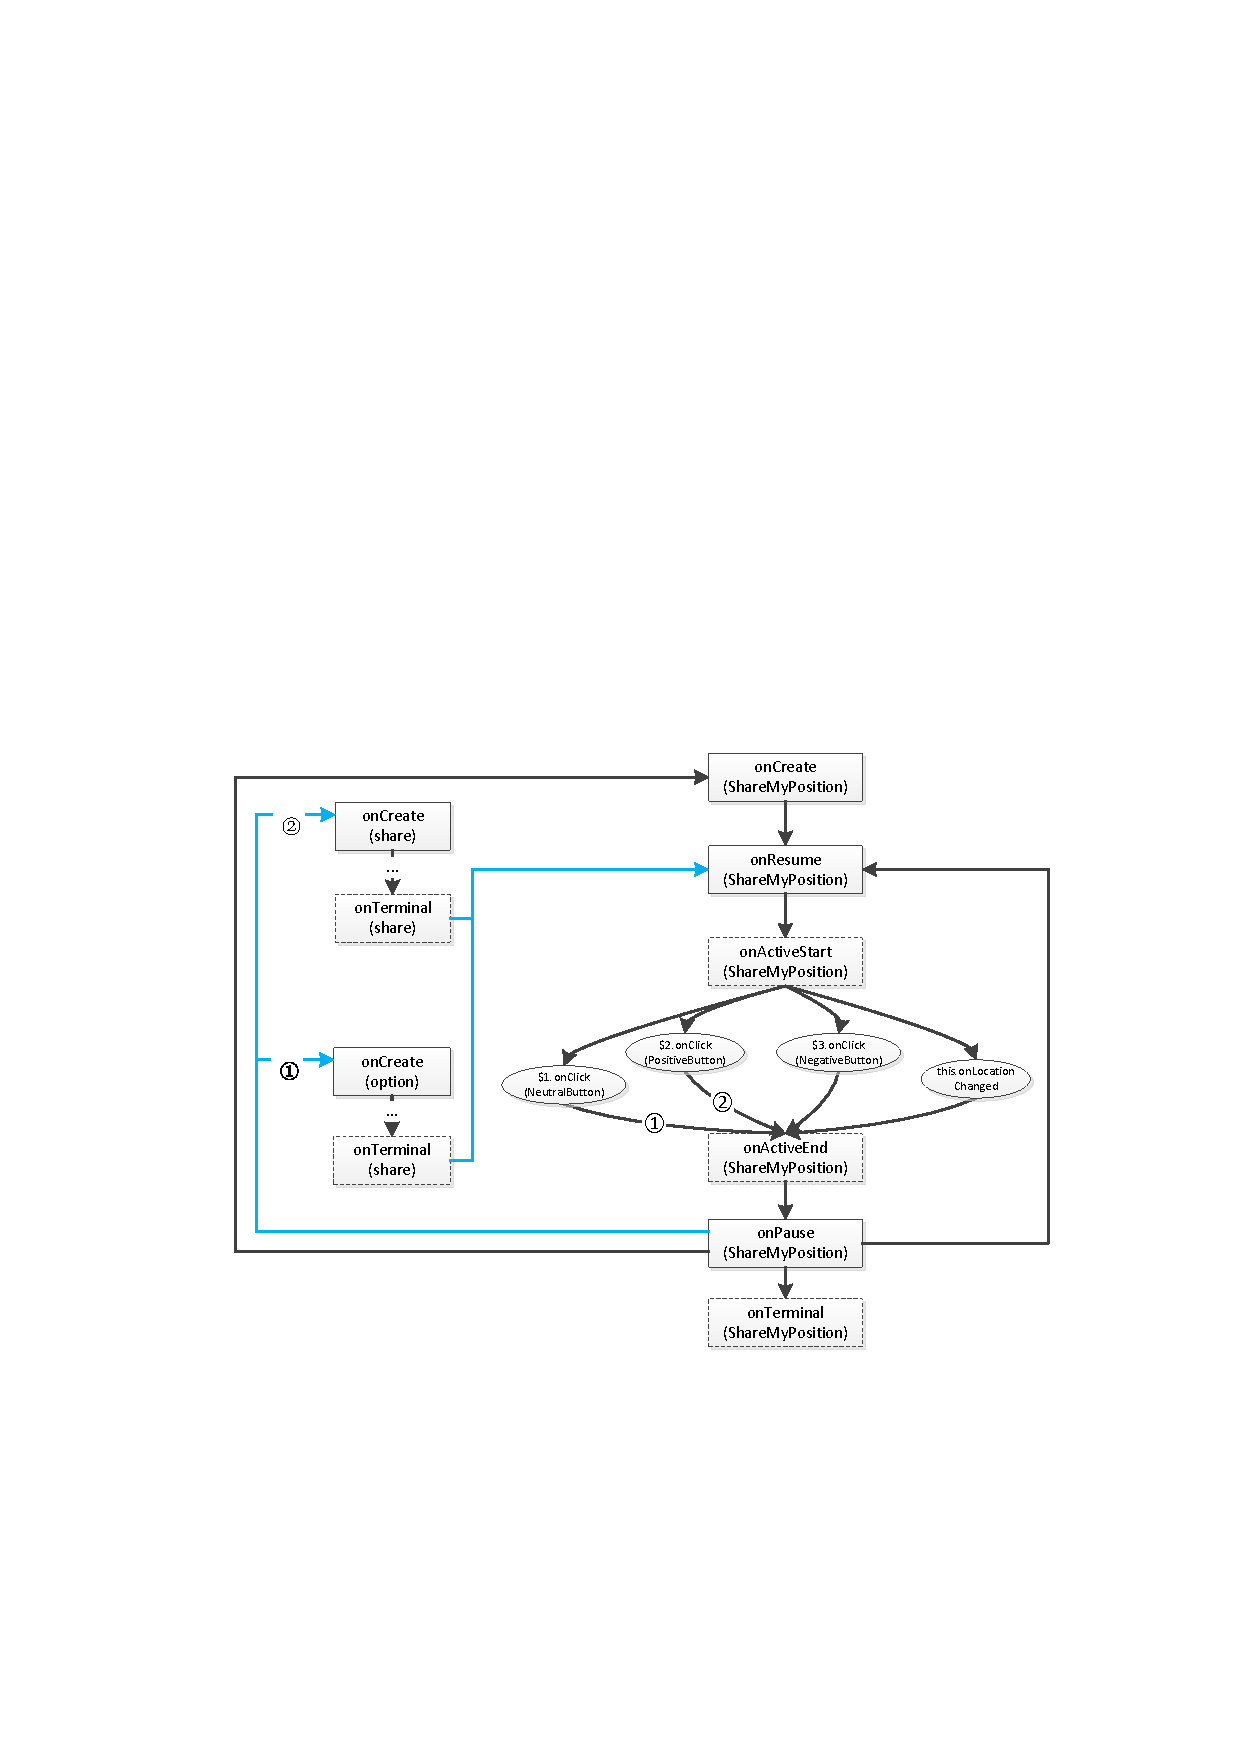
\includegraphics[width=1\linewidth]{pic/motivationGPM.pdf}  
%  \caption{GPC model illustration for motivation example.}  
%  \label{fig:motivationGPC}  
%\end{figure}

\begin{table*}[!t]
\centering
\begin{threeparttable}[b]
\caption{Path-sensitive conditions for motivation example. } 
\newcommand{\tabincell}[2]{\begin{tabular}{@{}#1@{}}#2\end{tabular}}
\small
\begin{tabular}{|c|c|c|c|c|}
\hline 
Node & Connection & ConType & Condition & Event\\ 
\hline 
\hline 
this.onCreate & \$1$::$onClick & FRA & N/A & env:(user,click,NeutralButton) \\ 
\hline 
this.onCreate & \$2$::$onClick & FRA & N/A & env:(user,click,PositiveButton) \\ 
\hline 
this.onCreate & \$3$::$onClick & FRA & N/A & env:(user,click,NegativeButton) \\ 
\hline 
this.onResume & this.onLocationChanged & FRA & \tabincell{c}{con:((v1 \&\& !v2)$\parallel$ \\
(v1 \&\& !v3))} &  env:(sys,locationChanged,locationManager)\\

\hline 
this.onPause & this.onLocationChanged & BRA & N/A & N/A \\ 
\hline 
this.onLocationChanged & this.onLocationChanged & BRA  & N/A & N/A \\ 
\hline 
\$1$::$onClick & option$::$onCreate & FJA  & N/A & N/A \\ 
\hline 
\$2$::$onClick & share$::$onCreate & FJA  & N/A & N/A \\ 
\hline 
\end{tabular}
\begin{tablenotes}
    \item [1] The signs \textit{v1}, \textit{v2} and \textit{v3} in column \textit{Condition} respectively refer to the variables \textit{containsGPS}, \textit{forceNetwork} and \textit{containsNetwork}
   \end{tablenotes}
\label{tbl: sensCond}  
\end{threeparttable}
\end{table*}
In this section, we introduce the \textit{GPC} construction algorithms, %Figure \ref{fig:motivationGPC} describes the \textit{GPC} model for the motivation example. 
including the following four stages.
%: 1) constructing path-insensitive inner component model, 2) constructing inter-component model, 3) constructing path-sensitive model and 4) handling fine-grained flow. %Correspondingly in Figure \ref{fig:motivationGPC} and Table \ref{tbl: sensCond}, the construction stages can be clearly mapped as: 1) constructing all the nodes and black edges; 2) constructing the blue edges; 3) obtaining the \textit{Conditions} column in Table \ref{tbl: sensCond}; 4) building the order numbers on Figure \ref{fig:motivationGPC}'s edges. Our approach is based on static analysis techniques. The input of our analysis algorithm is the app byte codes via reverse engineering. The output is the generated \textit{GPC} model, including the set of nodes, edges and conditions. Related conceptions have already been defined in Section \ref{transition-model}. 
%A conditionEdge can be a ordinary edge or the edge with trigger conditions that contains two parts: register conditions and trigger events.

\subsection{Path-insensitive Inner Component Model (\textit{PII})}
In this stage, we present a process\textit{ConsPII}. Taking the source code of a target component as its input, the process 
outputs a path-insensitive model for the component, including valid nodes (set \textit{N}) and edges between the nodes ($E_{l} \cup E_{r}$ -- lifecycle edges $E_l$ and register edges $E_r$).
%thow to construct the set of valid nodes \textit{N} and the set of edges $E_{l} \cup E_{r}$ (lifecycle and register edges) in each component. We call this process \textit{ConsPII}. As an improved static analysis, the algorithm takes the source code of the target component as its input. The output of \textit{ConsPII} is a path-insensitive model for target component, including valid nodes and edges. Since the set of nodes \textit{N} can be easily identified by matching pre-defined regular expression, \textit{ConsPII} focuses on constructing valid edges, namely the lifecycle edges $E_{l}$ and the register edges $E_{r}$.  

The nodes in \textit{N} are identified by matching pre-defined regular expression.
To compute $E_{l}$, \textit{ConsPII} first initializes an entire lifecycle graph (\textit{ELG}) in accordance with the type of the given component. Then, three \textit{auxiliary nodes} (\textit{onActiveStart}, \textit{onActiveEnd} and \textit{onTerminal}) are created and added into the ELG. They are used to explicitly mark the component status. \textit{ConsPII} then identifies the implemented lifecycle callback in the given component. For the nodes in the \textit{ELG} that are not implemented in the component, \textit{ConsPII} employs a displacement algorithm in the ELG, which involves three steps: 1) checking the pre-nodes and post-nodes of the unimplemented nodes, 2) generating edges connecting each pre-node with each post-node, 3) removing the unimplemented and its related edges. After the displacement, the $E_{l}$ is obtained from the remaining edges of ELG. 

%The $E_{r}$ are generated via identification of (un)register abstractions (\textit{RA}, defined in Section \ref{transition-model}).
To identify the edges in $E_r$, we first identify a set of register actions $\mathit{FRA}$, then the \textit{ConsPII} process adopts an improved \textit{DFS} (Deep First Search) algorithm over the entire program. The traversal process starts with \texttt{onCreate} callback in the launcher activity. For each identified register action $\mathit{fra}\in \mathit{FRA}$, the invokee callback \textit{ive} is taken as a new node and is inserted into \textit{active area} -- a lifecycle interval where the non-lifecycle callbacks are normally invoked. The \textit{active area} is defined for addressing the conflicts between lifecycle and non-lifecycle callbacks, and located between two auxiliary nodes: \textit{onActiveStart} and \textit{onActiveEnd}. There are two types of connections: \textit{lifecycle} $\rightarrow $ \textit{non-lifecycle} and \textit{non-lifecycle} $\rightarrow $ \textit{non-lifecycle}. The former generates edges \textit{onActiveStart} $\rightarrow $ \textit{ive} $\rightarrow $ \textit{onActiveEnd}; while the latter generates edges \textit{ivr} $\rightarrow $ \textit{ive} $\rightarrow $ \textit{onActiveEnd}, where \textit{ivr} is the invoker in the \textit{fra} tuple. %The black arrows and all the nodes in Figure \ref{fig:motivationGPC} are generated by \textit{ConsPII}. Note that in the figure, the \textit{onCreateDialog} is substituted by the \textit{onCreate}, since \texttt{onCreateDialog} is always invoked along with \textit{onCreate}, and thus can be treated as a part of it.

%\begin{algorithm}[!t]
%\caption{Connection between Components}
%\footnotesize
%\begin{algorithmic}[1]
%\Procedure {ConsPII} {$comp$}
%\State $ELG \leftarrow constructLifecycleGraph(comp)$
%\State $ auxNodes \leftarrow geneAuxNodes(comp)$
%\State $    nodes \leftarrow ELG.nodes$
%\State $    edges \leftarrow ELG.edges$
%\State $     lifeNodes, nonLifeNodes \leftarrow getAllValidCallbacks()$
%\ForAll {$hiddenNode \in (ELG.nodes \setminus lifeNodes)$}  
%\State $        edges \leftarrow edges \cup geneEdges(hiddenNode.preNodes,$\\
% $\ \ \ \ \ \ \ \        hiddenNode.postNodes)$
%\State $        nodes \leftarrow nodes \setminus hiddenNode$
%\State $        edges \leftarrow edges \setminus hiddenNode.edges$
%\EndFor

%\State $ FRA \leftarrow getRA(comp)$
%\ForAll {$ fra \in FRA $}
%\If {$fra.ivr\in lifeNodes\ \&\&\ fra.ive\in nonLifeNodes $}
%\State $            nodes \leftarrow nodes \cup fra.ive$
%\State $            edges \leftarrow edges \cup geneEdge(auxNodes.activeStart, fra.ive)$
%\State $            edges \leftarrow edges \cup geneEdge(fra.ive, auxNodes.activeEnd )$
%\ElsIf{$ fra.ivr\in nonLifeNodes\ \&\&\ $\\
% $\ \ \ \ \ \ \ \ \ \ \ \ \ \ \ \ \ \ fra.ive\in nonLifeNodes $}
%\State $  nodes \leftarrow nodes \cup fra.ive$
%\State $  edges \leftarrow edges \cup geneEdge(fra.ivr, fra.ive)$
%\State $  edges \leftarrow edges \cup geneEdge(fra.ive, auxNodes.activeEnd )$
%\Else {$ pass$}
%\EndIf
%\EndFor
%\EndProcedure
%\end{algorithmic}
%\label{fig:alg1}
%\end{algorithm}


%We use an improved DFS algorithm to traverse all the program source code (some irrelevant contents are excluded) and recognize the triple structure. The traversal process starts with the \texttt{onCreate} callback of launcher activity. First, system constructs a raw lifecycle model according to the lifecycle structure. This process is quite trivial. Then all the lifecycle callbacks in the raw model will be regarded as sub-roots, and each sub-root generates a flow-tree by linking the recognized the \textit{connection triple}. In this stage, we get a rough path-insensitive, control flow model. In this model, each callback acts as a node, and each connection triple acts as an edge.

%1) Checking register triple. Register triple determines when and where a callback becomes valid , as well as the connection between two related callbacks, especially the system-driven and user-driven callbacks. Checking the register triple is to find the execution sequences via traversing the program source code.

%2) Path-insensitive Inner Component Model. Inner component model acts as topology callback sequence without considering the connections of different components and jumping conditions. Constructing such model needs to well tackle the invocation order between lifecycle callbacks and other callbacks. Callback model generated in this step is able to represent fine-grained and complete callback sequences for each component.

%Algorithm 1 presents the analysis to detect registered actions. It essentially iterates over all program entry points (EntryPoints) and all actions (Action-Set) supported by the mobile framework (lines 6 􀀀 16). For each entry point P and action X it extracts the call graph of the app (line 5) and locates a set of statements PNodeSet (line 8) containing instances of a valid event-listener registering statement L for action X. Finally, for each statement PNode in PNodeSet it performs a backward slice on PNode to locate an initialization statement of the widget on which the instance of L was called (lines 10􀀀12). This is used to get an identier ID of the component (line 13) which is registered in the action map E with the action X.

\subsection{Connections between Components (\textit{CBC})}
Connections between components can be divided into two types: \textit{sequential jumping} and \textit{parallel jumping}. The former represents the invokee that occurs after the end of invoker. \textit{Sequential jumping} normally exists in the connections between activities, since the activities occupy the foreground (in running status) in sequence of invocation. The latter occurs when service involves, because a service runs in the background in parallel with the foreground activity or other services.

The process for constructing the connections is called \textit{ConsCBC} (Constructing the \textit{CBC}). \textit{ConsCBC} takes the sequential jumping as normal edges in \textit{PII}. As for parallel jumping, \textit{ConsCBC} generates specialized \textit{parallel edges} to represent the parallel relationship since it is beyond the representation of \textit{PII} and traditional \textit{CFG}. Typically, \textit{ConsCBC} considers the end connections (e.g., stopService, unbindService) as well as the start connections (e.g., startService, bindService). Specifically, if the trigger component is an activity, we define \textit{parallel slice} by the slice of a trigger activity model that can run in parallel with the service. For example, service \textit{S} is launched and stopped in activity \textit{A} via the API \texttt{startService} and \texttt{stopService}. Thus, only the nodes that can run between \texttt{startService} and \texttt{stopService} are possible to run in parallel with service \textit{S}. The paths consisting of such nodes and related edges in \textit{A} are treated as \textit{parallel slice}. The parallel slice provides a fine-grained picture for better understanding the parallel relation between the invoker and invokee. Algorithm \ref{fig:alg2} handles the parallel slice in line $16-25$. The algorithm traverses all the feasible paths that contain startNode (e.g., startService) and checks the paths that contain endNode (e.g., stopService) as well. Then, the algorithm marks the checked nodes as parallel slice nodes. Note that in parallel jumping, if the service is terminated by itself, the parallel slice will act as the entire \textit{PII} of trigger activity.

%\begin{algorithm}[!t]
%\caption{Path-insensitive Inner Component Model Construction}
%\footnotesize
%\begin{algorithmic}[1]
%\Procedure {ConsCBC} {$PII$, $connStSet$, $connEndSet$}
%\State $//Generate\ startConnection\ between\ component$
%\ForAll {$connSt \in connStSet$}  
%\If {$connSt\in activity\rightarrow activity$}
%\State $        geneEdge(connSt.holderNode, newCompEntry)$
%\ElsIf {$   connSt\in (comp \rightarrow service || service \rightarrow comp)  $}
%\State $        geneParallelEdge(connSt.holderNode, newCompEntry)$
%\Else $pass$
%\EndIf
%\EndFor
%\State $ //Generate\ endConnection\ between\ component $
%\ForAll {$ connEnd \in connEndSet $} 
%\State $  geneParallelEdge(service.end, connEnd.holderNode )$
%\EndFor    
%\State $ connPairSet\leftarrow Set(connSt.holderNode,connEnd.holderNode)$
%\State $       //Mark\ the\ parallel\ slice$
%\ForAll {$ connPair\in connPairSet$}
%\State $  pathsSt \leftarrow getPaths(connPair.startNode)$
%\ForAll {$ path in pathsSt $}
%\If { $ path.contains(connPair.endNode) $ }
%\State $   sliceNodes \leftarrow sliceNodes \cup path.nodes$
%\EndIf
%\EndFor
%\EndFor
%%\State $   // sliceNodes \leftarrow getSliceNodes(connPair)   //complexity\ is\ O(e)$
%\State $       markSliceNodes(sliceNodes )$
%\EndProcedure
%\end{algorithmic}
%\label{fig:alg2}
%\end{algorithm}


%Components of different types can be executed in parallel, which is beyond the representation of existing modelling approaches. For example, if a service \textit{s} is launched by an activity \textit{a}, the \textit{s} will run it program logic in background, and this time the foreground \textit{a} continues its running. 

%The GPC model can represent this relationship through \textit{parallel slice} of the trigger component. The \textit{parallel slice} is from a trigger node to a close node, which respectively trigger other component active and destroy. The triggered component only can be executed parallel with the logic with \textit{parallel slice} of the trigger component. Some components are triggered or closed by themselves. For example, a statically registered broadcastreceiver is triggered when the app starts; a service destroys its process by itself. The \textit{parallel slice} of activities (if any) for these components are the entire activities program. GPC model uses different flags to sign the different \textit{parallel slices}.

%3) Connections of Components. The generated models by steps 2 aiming to single component can not reflect invocation relations for entire app program. The connections of components focuses on both new component trigger and stop. Especially, in connecting with the parallel (可并行的) component like service, the specific \textit{parallel slice } is computed through the feasible path nodes between trigger and stop point.

\subsection{Path-sensitive Inter-component Model (\textit{PSI})} 
The \textit{PII} and \textit{CBC} lack identification for trigger conditions, which heavily limits the available area. To address this issue, a path-sensitive modelling approach called \textit{ConsPSI} (constructing the \textit{PSI}) has been proposed, as shown in Algorithm \ref{fig:alg3}. Essentially, \textit{ConsPSI} aims at handling the trigger conditions for registering edges $E_{r}$ and inter-component connections $E_{j}$. Lifecycle edges $E_{l}$ need not to be handled since they are triggered without extra conditions. For each edge in $E_{r}$ and $E_{j}$, the path-sensitive model represents the condition set under which the invokee callback is fired. To achieve this goal, \textit{ConsPSI} engages a backward data dependency analysis for critical program slice, which involves two core analyses: \textit{checkCV} (for checking the condition variables) and \textit{backTraverse} (for tracking the condition values). Since \textit{ConsPSI} uses the same methods to handle $E_{j}$ as to handle $E_{r}$, we only describe how to handle $E_{r}$ for simplification.

The goal of \textit{checkCV} is to check the trigger conditions for callback invocation and to record variable set within such conditions. The checked objects intuitively originate from the register action (\textit{rAct}) contained in \textit{FRA}, because the invocation of a non-lifecycle callback heavily relies on execution of the \textit{rAct}. For each $fra\in FRA$, \textit{checkCV} identifies the \textit{rAct} branch using backward matching, and then records the branch conditions. In essence, \textit{checkCV} abstracts all the variables within the branch conditions and preserves them in a maintained list \textit{CVList}.

The \textit{backTraversal} for variable dependency analysis is based on the \textit{CVList} obtained by \textit{checkCV}. The goal for \textit{backTraversal} is to clarify the values of condition variables. To this end, \textit{backTraversal} backward tracks the variable assignment to update the \textit{CVList}. The atomic unit of \textit{CVList} is a variable tuple $\textit{vt} = (var, val)$, where \textit{var} and \textit{val} refer to the name and value of the variable. The \textit{val} can be either a \textit{vt} set or a terminal value. The tuple \textit{vt} keeps evolving during variable tracking. Eventually, all the \textit{val}s in \textit{vt} are updated to terminal values. The evolving process of motivation example is shown in Figure \ref{fig:motConds}. Leaves \textit{vt}s (blue nodes) in Figure \ref{fig:motConds} only contain terminal values. Typically, \textit{backTraversal} records three types of leaf \textit{val} at the end of tracking: constant value, \textit{PARA} and \textit{GLOBAL}. \textit{PARA} and \textit{GLOBAL} represent the parameter type and global type of \textit{var}, respectively. When the tracking ends in a method, the \textit{val} is still possible to be an undetermined variable. \textit{backTraversal} identifies the types of these variables and marks them as \textit{PARA} or \textit{GLOBAL}. The implementation process of \textit{backTraversal} is shown in Algorithm \ref{fig:alg3} line $4-11$. Eventually, the final results stored in \textit{pathSens} are treated as an attribute of the invoker node in $fra$.

%For each item in \textit{CVList}, \textit{backTraversal} iteratively backward tracks its assignment site and stores it in a defined\textit{pathSens} list. If the assignment contains new variables, add them into \textit{CVList} and repeat the tracking. 


The path-sensitive condition determines whether a callback is active; while the trigger event determines whether it is invoked.
\textit{ConsPSI} gets the corresponding trigger event tuple (Definition 4) in accordance to the invokee type, and then assigns the tuple to the invoker node as its attribute. 


\textit{Limitations.}
Currently, the path-sensitive model only supports intra-procedural condition tracking, which limits the precision of condition values. In fact, inter-procedural data dependency analysis exploits similar method in tracking the variables as the intra one. The differences embody in the process of handling the parameters. However, it requires extra costs to handle the inter-procedural data tracking. How to improve the precision of inter-procedural condition tracking in an acceptable time and resource cost is a direction of our future works.


%\begin{figure}[!t]  
%  \centering  
%  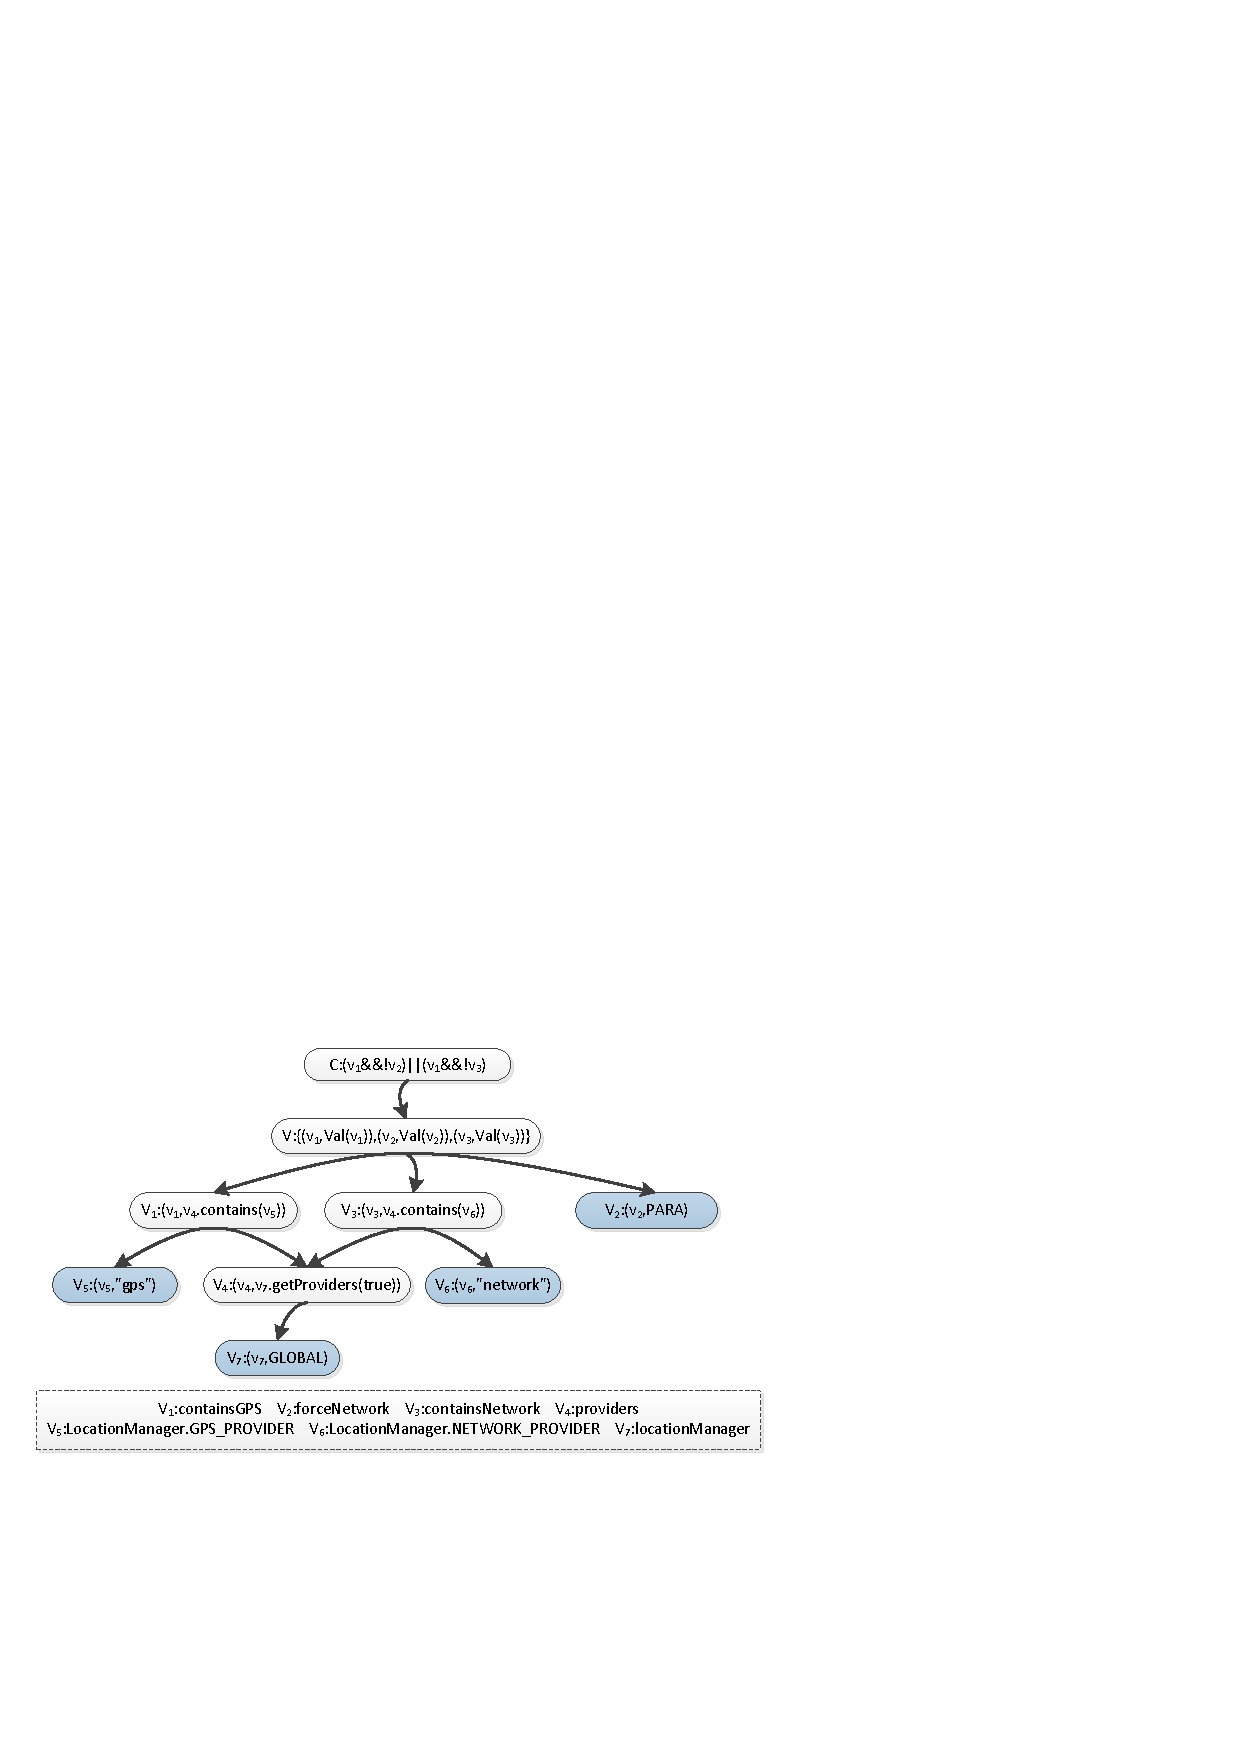
\includegraphics[width=1\linewidth]{pic/motivationCondition.pdf}  
%  \caption{Process of path-sensitive condition for motivation example.}  
% \label{fig:motConds}  
%\end{figure}

%\begin{algorithm}[!t]
%\caption{Path-sensitive Inter-component Model Construction}
%\footnotesize
%\begin{algorithmic}[1]
%\Procedure {ConsPSI} {$PII_SET$, $FRA$}
%\ForAll {$ rra \in FRA $}        
%\State $          CVList \leftarrow checkCV(fra.registerSite ) $
%\While {$\not CVList.empty$}     
%\State $                 var \leftarrow CVList.pop(0)$
%\State $                 assignSite \leftarrow backTraversal(var)$
%\State $                 pathSens \leftarrow pathSens \cup (var, assignSite )$
%\If{ $assignSite.hasNewVars$ }
%\State $                     CVList \leftarrow CVList \cup assignSite.newVars$
%\EndIf
%\EndWhile    
%\State $           fra.ivr.attr \leftarrow fra.ivr.attr \cup pathSens $
%\State $           fra.ivr.attr \leftarrow fra.ivr.attr \cup getTriggerEvent(fra.ive)$
%\EndFor
%\EndProcedure
%\end{algorithmic}
%\label{fig:alg3}
%\end{algorithm}

%If a non-lifecycle callback status is active, namely St1(c)-> {active}, its register point has already been executed, namely Rt1(c)->{executed}. And vice versa. That means the status of non-lifecycle callback is determined by the execution status of corresponding register point. Therefore, instead analyzing the target callback, we choose to check the execution condition of corresponding register point. 
%We use back-check to find the branch structure and the condition content, referenced by CC, of target register point. For the obtained CC, we abstract the variables set, referenced by V. For each variable in V, we do \textit{backTraversal} data dependency analysis. 

%We store the variable as a triple (type, name, value), which is named \texttt{condTriple}. Initially, the \textit{type} and \textit{value} are set as \texttt{null}. We only concern certain types of condition variables, which shown in Figure 3. For other unknown types, we use \texttt{u} to denote them.

%The \textit{backTraversal} checks the nearest assignment along the backward of the program. Then the \textit{type} and \textit{value} are assigned as the right-value. If the right-value is a new variable, the \textit{value} of the triple will be expanded as new triple set. The \textit{backTraversal} continues the process for right-value until reaching an end point without a empty \textit{value}.

%The analyses update the condTriple for each statement in a method until a fixed point is reached. For inter-procedural cases, the \textit{backTraversal} exploits method summary to describe the data flow information within a typical method. Methods are analyzed in reverse topological order with respect to the app system’s call graph. Thus, the entire app system can be analyzed.  

%4) Path-sensitive Model. Prior work lacks handling of path-sensitive issues. However, path-sensitive modelling improvements precision of {\color{red}both program flow and model traversing}, and further, provide assistance for related research like model checking and test case generation. Path-sensitive in modelling GPC model concerns valiables and their values that can impact the active status of succeed callbacks. 

%Although traditional IFDS \cite{} considers the interprocedural and distributive problems. It is still hard to cover the problem how and when to trigger an existing callback function. In Android framework, this problem is of particular importance causing the general existence of callbacks that directly determines a program execution direction. 

%2) In theory, a non-lifecycle callback is invoked under two conditions. One is its register-site is executed; the other is the trigger event fires. In this way, a non-lifecycle callback is possible to be invoked during running of any lifecycle callback, when satisfies the two conditions. Here we don't consider 

\subsection{Jumping Confusion}\label{jumpConfusion}
% If a lifecycle callback is not implemented in the real app, it is called hidden node. In our GPC model model, hidden node will not be represented, instead of corresponding edges. For a hidden node, all its in-edges connect all its out-edges. For example, in the \texttt{onPause} acts as a hidden node, it has one in-edge (from \texttt{onResume}) and three out-edges (to \texttt{onCreate}, \texttt{onStop} and \texttt{onResume} itself). Thus, there would be three extra edges generated by GPC model, respectively \texttt{onResume} to \texttt{onCreate},  \texttt{onResume} to \texttt{onStop} and \texttt{onResume} to itself.
In activity jumping edges $E_{j-a}$, multiple jumping invokers $subIvr\subseteq Ivr\in JA$  existing in the same activity would result in \textit{jumping confusion} (mentioned in Section \ref{problem-define}). A naive solution is to generate a direct edge connecting the invoker \textit{ivr} with invokee \textit{ive}. However, this solution ignores the related lifecycle nodes (i.e., \texttt{onActiveEnd} and \texttt{onPause}) in real sequence. Our analysis adopts a marking algorithm to address the jumping confusion. For each jumping edge $E_{j-a}$, we use a unique ID to mark the edge from its \textit{ivr} to the \textit{onActiveEnd} node, and then the same ID is used to mark the edge from \textit{onPause} node to its \textit{ive}. If two jumping actions point to the same \textit{ive}, they share the same ID. An illustration example is shown in Figure \ref{fig:motivationGPC}. The edges $\$1.onClick\rightarrow shareMyPosition.onActiveEnd$ and $shareMyPosition.onPause\rightarrow option.onCreate$ are marked as ID $1$, and other two similar edges are marked as ID $2$.

%For example, when an activity \textit{a1} jumps to another one \textit{a2}. It has to pass by the \texttt{onPause} and \texttt{onStop} callbacks, whatever callback, referenced by \textit{c1}, the jump logic is located. To this end, there should be an edge connecting the \textit{c1} and  \texttt{onPause} node. Analogously, another edge should connect the \texttt{onStop} to \textit{a2}'s \texttt{onCreate}, as shown in Figure 4. However, it is unreasonable that the path c1->onPause->onStop->a3. To address this issue, we define signed edge. 
\textit{Traversal Strategy.} 
Model traversal adopts the following strategy to avoid jumping confusion. If a traversal iterator passes an edge marked \textit{n}, then it is restricted to run along with either an unmarked edge, or an edge marked \textit{n}. After the iterator passes the jumping edge, the above restriction is removed.

%This way can effectively distinguish the callback flow in jumping logic without redundancy (without the signed edge, it has to create redundant \texttt{onPause} or \texttt{onStop} node).

%If a system-driven callback does not unregister before jumping to a new activity, then the callback is still active in the new activity states. Here we don't consider such situation.








  


%\Procedure {BellmanKalaba}{$G$, $u$, $l$, $p$}
%\ForAll {$v \in V(G)$}
%\State $l(v) \leftarrow \infty$
%\EndFor
%\State $l(u) \leftarrow 0$
%\Repeat
%\For {$i \leftarrow 1, n$}
%\State $min \leftarrow l(v_i)$
%\For {$j \leftarrow 1, n$}
%\If {$min > e(v_i, v_j) + l(v_j)$}
%\State $min \leftarrow e(v_i, v_j) + l(v_j)$
%\State $p(i) \leftarrow v_j$
%\EndIf
%\EndFor
%\State $l’(i) \leftarrow min$
%\EndFor
%\State $changed \leftarrow l \not= l’$
%\State $l \leftarrow l’$
%\Until{$\neg changed$}
%\EndProcedure
%\Statex
%\Procedure {FindPathBK}{$v$, $u$, $p$}
%\If {$v = u$}
%\State \textbf{Write} $v$
%\Else
%\State $w \leftarrow v$
%\While {$w \not= u$}
%\State \textbf{Write} $w$
%\State $w \leftarrow p(w)$
%\EndWhile
%\EndIf
%\EndProcedure


%\begin{figure}[htb]
%  \centering  
%   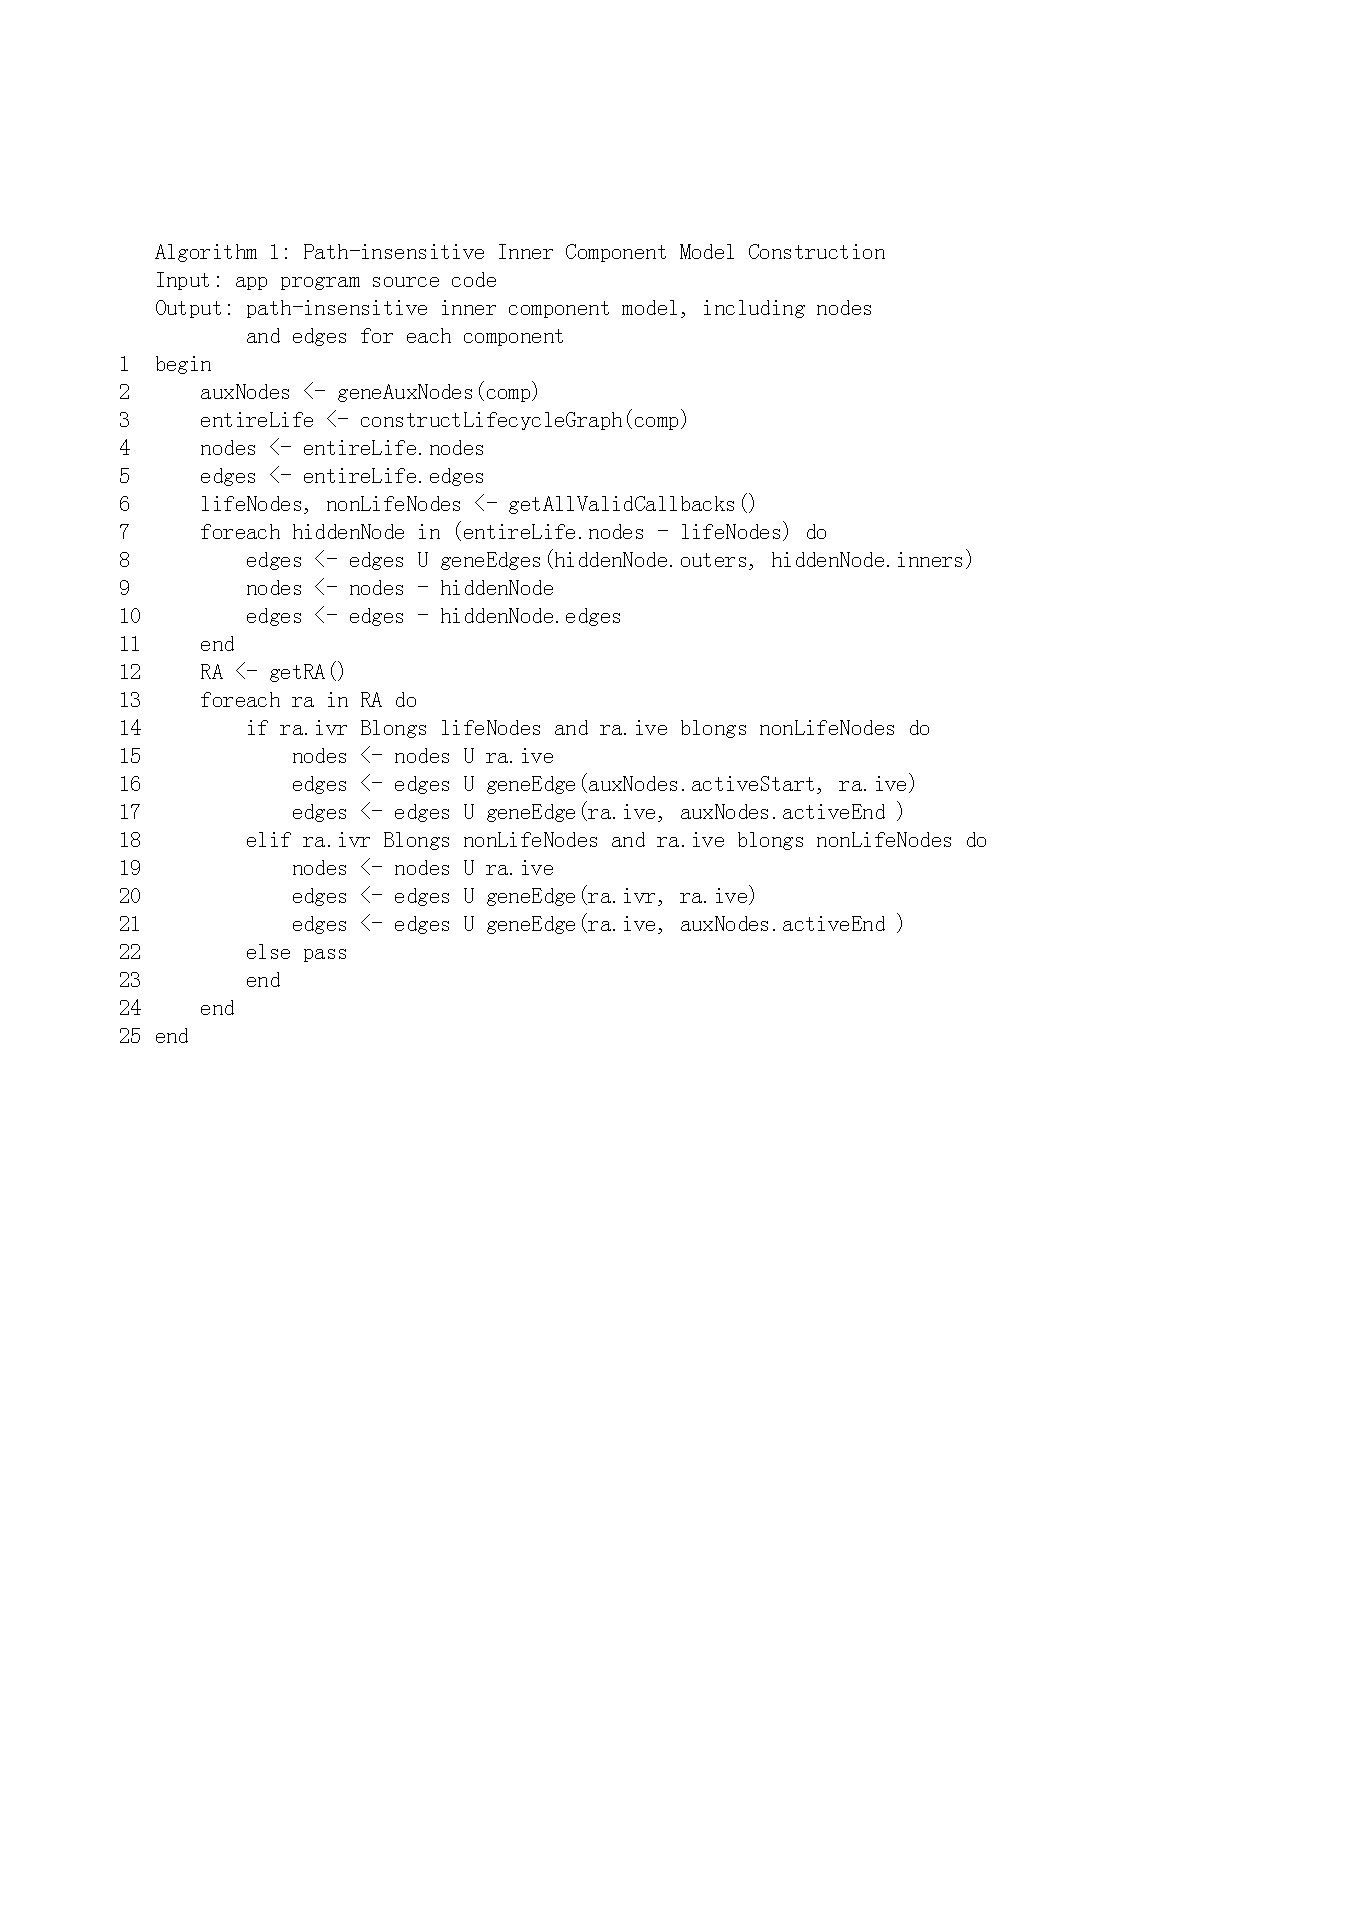
\includegraphics[width=1\linewidth]{pic/Algorithm1.pdf}   
%   %\caption{Some description about the picture}
%   \label{fig:alg1}
%\end{figure}

%\begin{figure}[htb]
%  \centering  
%   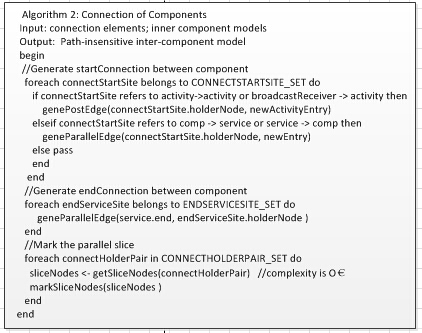
\includegraphics[width=1\linewidth]{alg2.jpg}   
%   %\caption{Some description about the picture}
%   \label{fig:alg2}
%\end{figure}

%\begin{figure}[htb]
%  \centering  
%   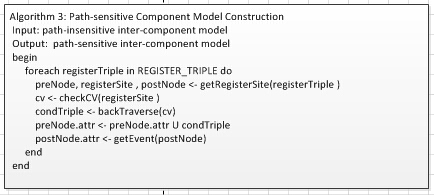
\includegraphics[width=1\linewidth]{alg3.jpg}   
%   %\caption{Some description about the picture}
%   \label{fig:alg3}
%\end{figure}
